\chapter{Implementasi Dan Pengujian Aplikasi}
\label{chap:implementasi dan pengujian aplikasi}

Pada bab 5 akan dibahas implementasi dan pengujian aplikasi pembuatan \textit{Twitter bot} untuk mencari jalur transportasi publik.

\section{Lingkungan Pembangunan}
Lingkungan perangkat lunak dan perangkat keras yang digunakan untuk membangun dan menguji aplikasi pembuatan \textit{Twitter bot} untuk mencari jalur transportasi publik ini adalah:
\begin{itemize}
	\item Komputer
	
	
	\begin{itemize}
		\item Processor: Intel Core i7-2630QM CPU 2.00 GHz
		\item RAM: 4096MB
		\item Hardisk: 211GB
		\item VGA : NVDIA GeForce GT 540M
	\end{itemize}
	\item Sistem operasi: Windows 7 Professional
	\item Platform: NetBeans: IDE 8.0.2
	
	\item Akun \textit{Twitter bot}
	\begin{itemize}
		\item Nama akun: kviniink
		\item ConsumerKey : 3iT8duMItTTrdaU1qTHxwDIUl
		\item ConsumerSecret : YUIgJTbQT3i5tYA5RE0L38dPT9HaDhuBTifvVmKDYeOgJ7t313
		\item AccessToken : 313287708-NO5SPbreQvoOxtXUD5EcKlubIfCBNfCb6aRqYBlZ
		\item AccessTokenSecret : LVfDgtlfeht5yjBJGSgvSvtMYcFMoEdYOspYoOptcuR4i
	\end{itemize}
	
	\item Akun Twitter penguji : kviniinktest123
\end{itemize}


\section{Hasil Penggunaan Antarmuka}
Pembuatan perangkat lunak \textit{Twitter bot} untuk mencari jalur transportasi publik ini memiliki tampilan antarmuka berbasis teks yang berguna untuk melihat hasil \textit{tweet} yang diterima \textit{Twitter bot}, dan hasil \textit{tweet} yang di-\textit{reply} \textit{Twitter bot} kepada pengguna. Gambar~\ref{fig:antarmukaProgram} adalah tampilan antarmuka \textit{Twitter bot} untuk mencari jalur transportasi publik.

\begin{figure}
	\centering
		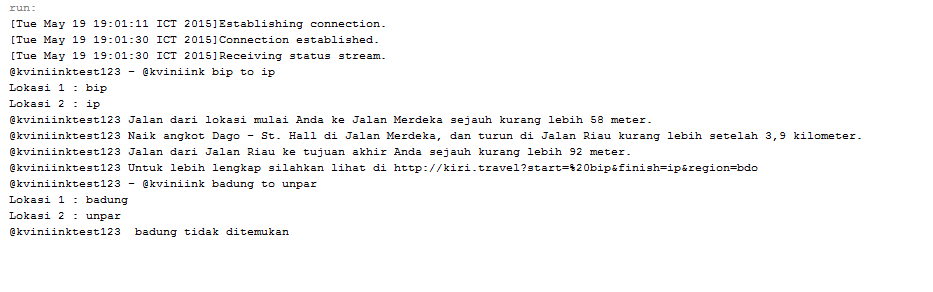
\includegraphics[width=0.75\textwidth]{C:/Skripsi/doc/DokumenSkripsi/Gambar/antarmukaProgram.PNG}
	\caption{Antarmuka Perangkat Lunak Twitter Bot Untuk Mencari Jalur Transportasi Publik}
	\label{fig:antarmukaProgram}
\end{figure}

\paragraph{Antarmuka Twitter}
Pengguna dapat mencoba perangkat lunak \textit{Twitter bot} menggunakan Twitter, baik menggunakan \textit{website} Twitter ataupun aplikasi Twitter. Oleh karena itu, tampilan antarmuka setiap pengguna akan berbeda-beda sesuai dengan \textit{device} yang digunakan pengguna. Berikut adalah contoh beberapa tampilan antarmuka yang diberikan oleh Twitter:

\begin{itemize}
	\item Antarmuka Twitter yang diakses melalui aplikasi Twitter di Android dapat dilihat pada Gambar~\ref{fig:TwitterAndroid}
			
			\begin{figure}[htbp]
				\centering
					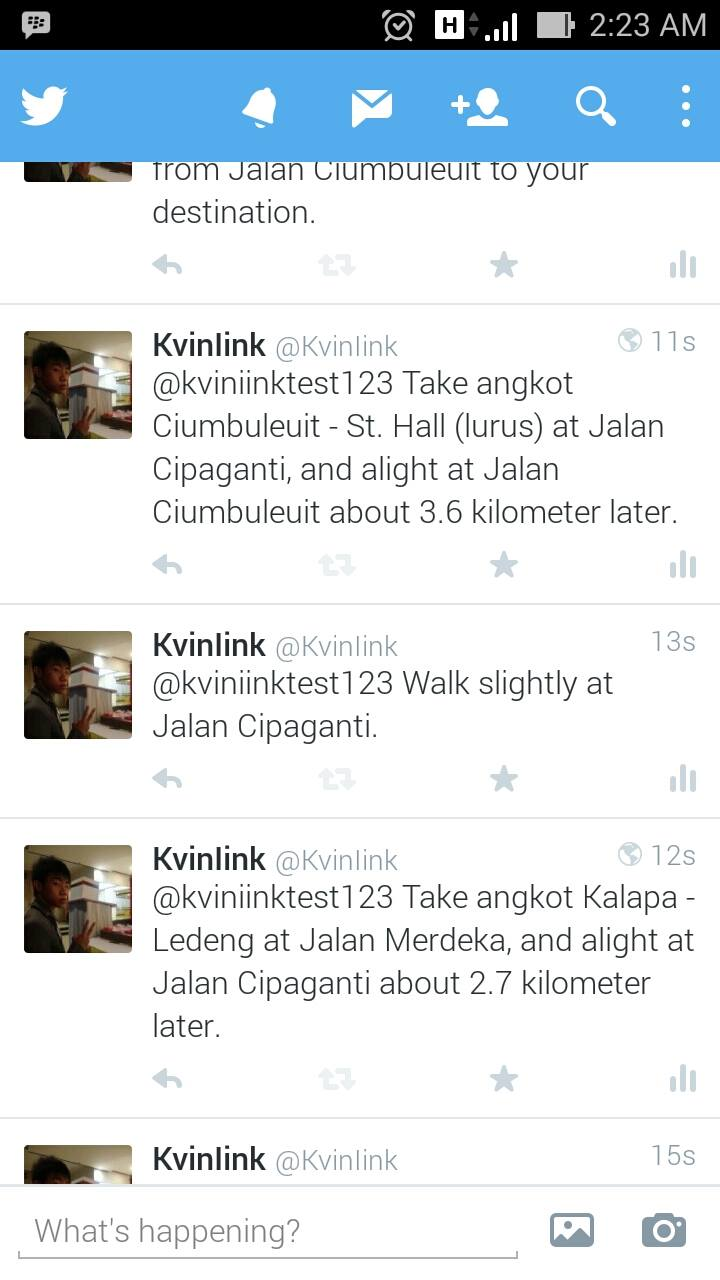
\includegraphics[width=0.5\textwidth]{C:/Skripsi/doc/DokumenSkripsi/Gambar/TwitterAndroid1.jpg}
				\caption{Antarmuka Twitter yang diakses melalui aplikasi Twitter di Android}
				\label{fig:TwitterAndroid}
			\end{figure}
			
	\item Antarmuka Twitter yang diakses melalui aplikasi Twitter di iOS dapat dilihat pada Gambar~\ref{fig:TwitteriOS}
	
	
	\begin{figure}[htbp]
		\centering
			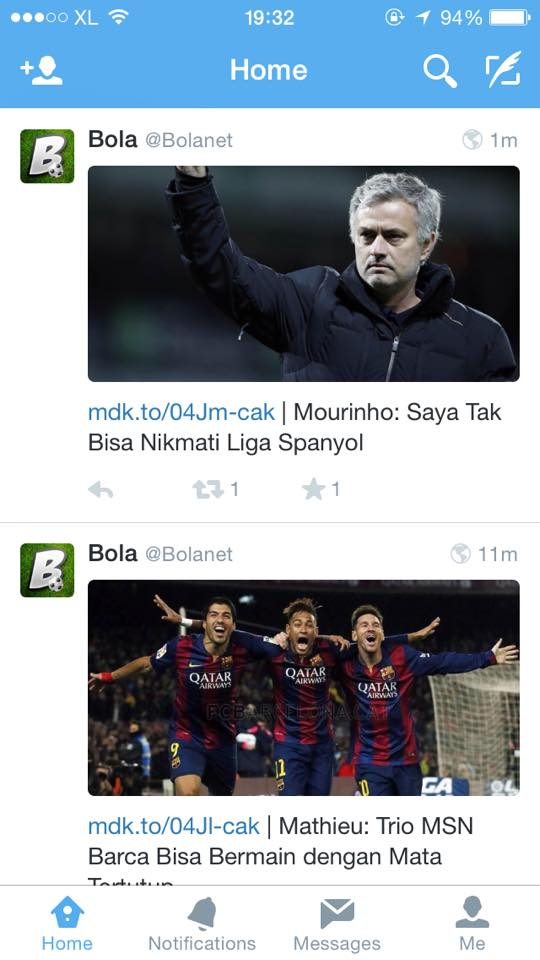
\includegraphics[width=0.5\textwidth]{C:/Skripsi/doc/DokumenSkripsi/Gambar/TwitteriOS.jpg}
		\caption{Antarmuka Twitter yang diakses melalui aplikasi Twitter di iOS}
		\label{fig:TwitteriOS}
	\end{figure}
	
	\item Antarmuka Twitter yang diakses melalui aplikasi Twitter di Windows Phone dapat dilihat pada Gambar~\ref{fig:TwitterWP}
	
	
	\begin{figure}[htbp]
		\centering
			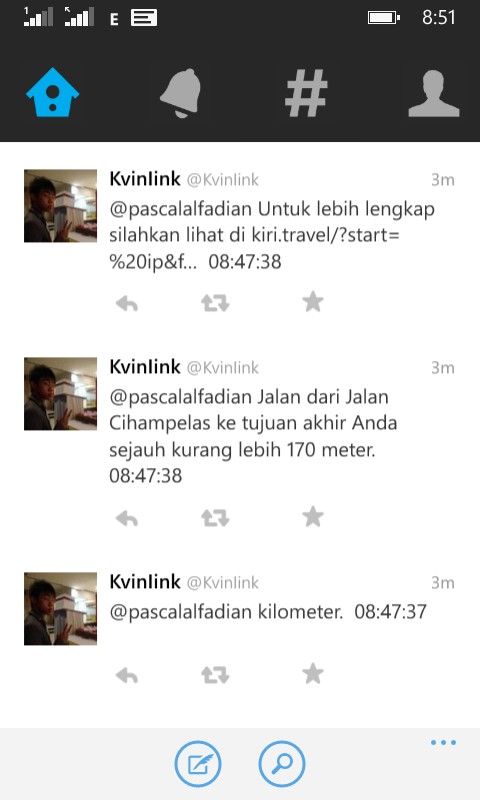
\includegraphics[width=0.5\textwidth]{C:/Skripsi/doc/DokumenSkripsi/Gambar/TwitterWP.jpg}
		\caption{Antarmuka Twitter yang diakses melalui aplikasi Twitter di Windows Phone}
		\label{fig:TwitterWP}
	\end{figure}
	
	
	\item Antarmuka Twitter yang diakses melalui aplikasi Twitter di Website Twitter dapat dilihat pada Gambar~\ref{fig:homePageTwitter}

	
	\begin{figure}[htbp]
		\centering
			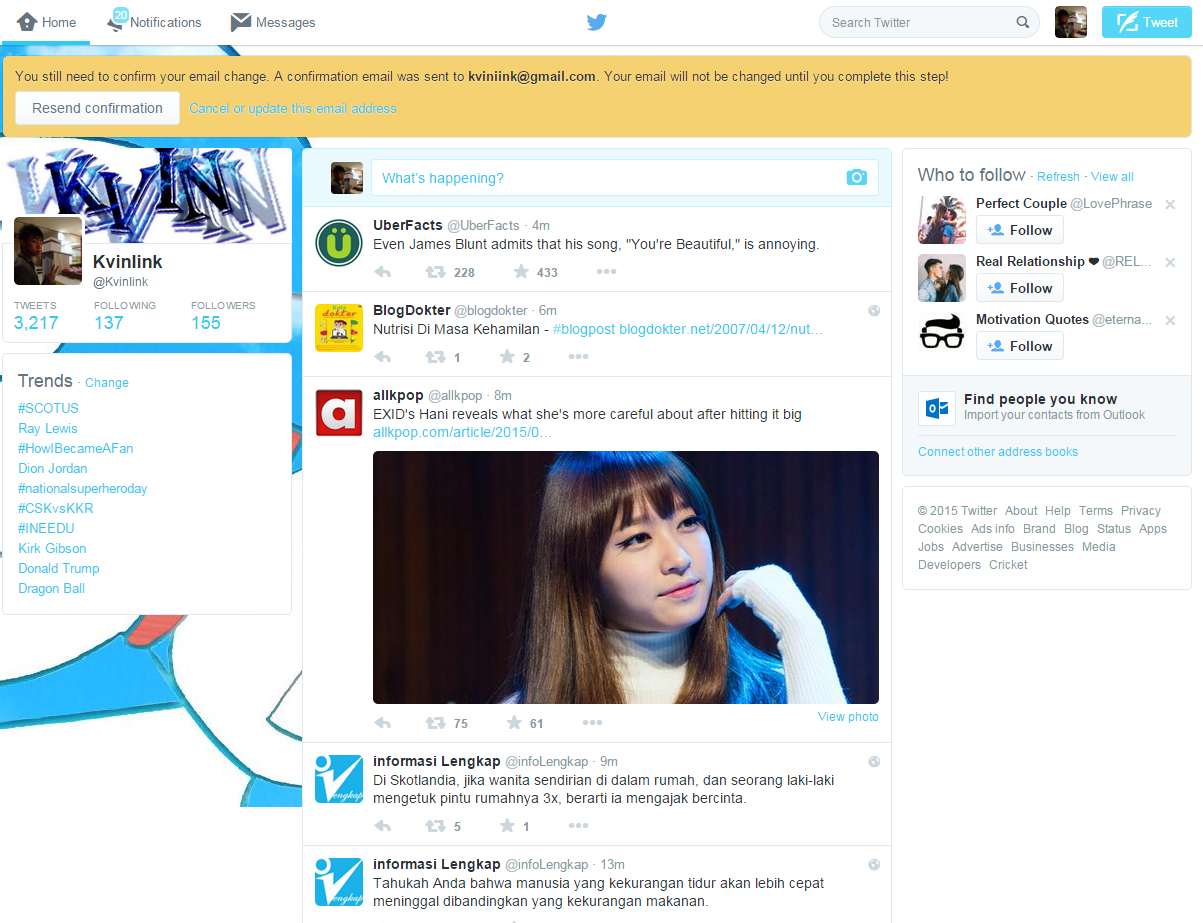
\includegraphics[width=0.75\textwidth]{C:/Skripsi/doc/DokumenSkripsi/Gambar/homePageTwitter.PNG}
		\caption{Antarmuka Twitter yang diakses melalui aplikasi Twitter di Website Twitter}
		\label{fig:homePageTwitter}
	\end{figure}
	
\end{itemize}

\iffalse
Tampilan \textit{home page} Twitter dapat dilihat pada Gambar~\ref{fig:Homepage Mobile Twitter}. Disini peneliti menggunakan website Twitter versi mobile agar lebih mudah dilihat karena tampilan website Twitter versi mobile lebih sederhana dibandingkan website Twitter versi desktop. Setelah itu user akan menekan tombol \textit{tweet} pada pojok kanan atas dan akan memberikan tampilan seperti pada Gambar~\ref{fig:Textbox Mobile Tweet}. Dari situ user dapat melakukan \textit{tweet} kepada \textit{Twitter Bot} untuk mencari jalur transportasi publik.
\begin{figure}[htbp]
	\centering
		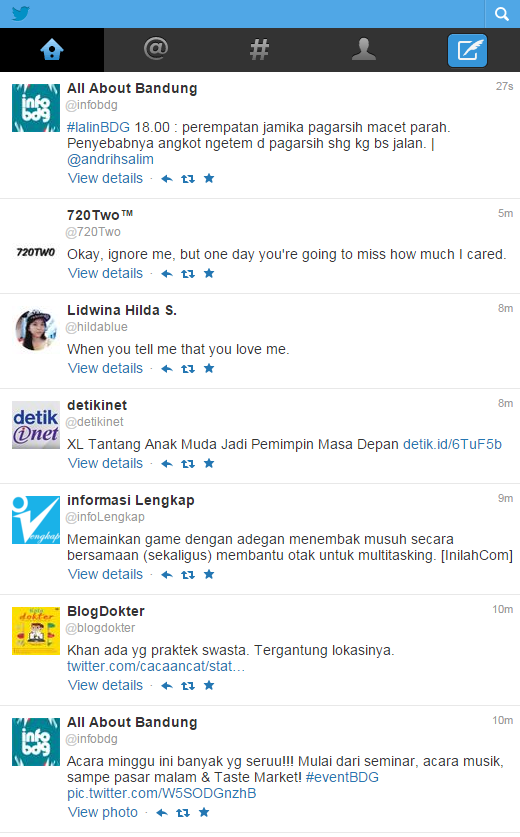
\includegraphics[width=1.00\textwidth]{C:/Skripsi/doc/DokumenSkripsi/Gambar/Homepage Mobile Twitter.PNG}
	\caption{Homepage Twitter versi mobile}
	\label{fig:Homepage Mobile Twitter}
\end{figure}


\begin{figure}[htbp]
	\centering
		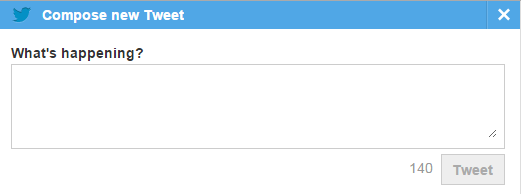
\includegraphics[width=1.00\textwidth]{C:/Skripsi/doc/DokumenSkripsi/Gambar/Textbox Mobile Tweet.PNG}
	\caption{Tampilan untuk melakukan \textit{tweet}}
	\label{fig:Textbox Mobile Tweet}
\end{figure}

Setelah ada \textit{mention} yang ditujukan kepada \textit{Twitter Bot}, aplikasi akan menangkap \textit{tweet} tersebut dan ditampilkan dalam bentuk pesan \textit{tweet} yang diterima oleh aplikasi. Hasil \textit{tweet} yang diterima aplikasi dapat dilihat pada Gambar~\ref{fig:HasilTangkapanTweetBerbasisTeks}. Setelah itu \textit{tweet} akan diperiksa oleh aplikasi apakah \textit{tweet} tersebut bertujuan untuk mencari jalur transportasi publik atau tidak. Jika benar, maka aplikasi akan melakukan proses pencarian jalur transportasi publik dan melakukan \textit{reply} atau balasan kepada pengguna. \textit{Reply tweet} tersebut berisikan jalur transportasi publik yang harus ditempuh kepada \textit{user}. Selain melakukan \textit{reply}, aplikasi juga menampilkan \textit{tweet} tersebut yang dapat dilihat pada Gambar~\ref{fig:HasilTweetBerbasisTeks}.

\begin{figure}
	\centering
		
\includegraphics{C:/Skripsi/doc/DokumenSkripsi/Gambar/HasilTangkapanTweetBerbasisTeks.PNG}
	\caption{Hasil streaming \textit{tweet}}
	\label{fig:HasilTangkapanTweetBerbasisTeks}
\end{figure}

\begin{figure}
	\centering
		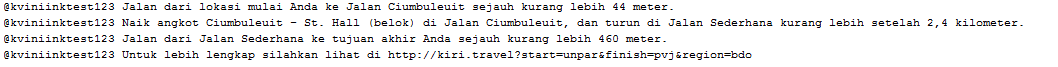
\includegraphics{C:/Skripsi/doc/DokumenSkripsi/Gambar/HasilTweetBerbasisTeks.PNG}
	\caption{Hasil balasan \textit{tweet} kepada user}
	\label{fig:HasilTweetBerbasisTeks}
\end{figure}
\fi

\newpage
\section{Pengujian}
Pada sub-bab ini akan dibahas mengenai hasil pengujian yang telah dilakukan terhadap perangkat lunak yang dibangun oleh penulis. Pengujian terdiri dari dua bagian, yaitu pengujian fungsional dan pengujian eksperimental. Pengujian fungsional bertujuan untuk memastikan semua fungsi aplikasi berjalan sesuai harapan. Sementara pengujian eksperimental bertujuan untuk mengetahui keberhasilan proses kerja dari aplikasi yang dibangun.

\subsection{Pengujian Fungsional}
Pengujian fungsional dilakukan pada fungsionalitas yang tersedia pada aplikasi yang dibangun. Pengujian ini dilakukan untuk mengetahui kesesuaian reaksi nyata dengan reaksi yang diharapkan dari aplikasi yang dibangun. Hasil pengujian ditunjukan pada tabel ~\ref{tab:TabelHasilPengujianFungsionalitasPadaAplikasiTwitterBotUntukMencariJalurTransportasiPublik}.

\begin{table}[h]
	\caption{Tabel Hasil pengujian fungsionalitas pada Aplikasi \textit{Twitter bot} untuk mencari jalur transportasi publik}
	\label{tab:TabelHasilPengujianFungsionalitasPadaAplikasiTwitterBotUntukMencariJalurTransportasiPublik}
		\begin{tabular}{|p{0.5cm}|p{3cm}|p{5cm}|p{5cm}|}
			\hline
				No & Pengujian & Reaksi yang Diharapkan & Reaksi Aplikasi  \\ \hline
				1 & Melakukan otentikasi terhadap akun \textit{Twitter Bot} & Otentikasi berhasil dilakukan antara Twitter dengan akun \textit{Twitter Bot}. Otentikasi dilakukan dengan melakukan pemeriksaan terhadap \textit{ConsumerKey}, \textit{CustomerSecret}, \textit{AccessToken}, dan \textit{AccessTokenSecret} &  \textit{ConsumerKey}, \textit{CustomerSecret}, \textit{AccessToken}, dan \textit{AccessTokenSecret} yang diberikan Twitter berhasil diotentikasi oleh aplikasi \\ \hline
				2 & Melakukan \textit{streaming tweet} & Menangkap semua \textit{tweet} yang di\textit{mention} kepada akun @kviniink & Setiap \textit{tweet} yang di\textit{mention} kepada akun \textit{Twitter bot} @kviniink dapat diterima secara \textit{realtime}\\ \hline
				3 & Membaca \textit{tweet} yang ditangkap & Melakukan pemeriksaan terhadap \textit{tweet} yang ditangkap, apakah \textit{tweet} tersebut merupakan \textit{tweet} untuk mencari transportasi publik atau bukan & Perangkat lunak dapat membedakan \textit{tweet} untuk mencari jalur transportasi publik dengan \textit{tweet} yang bukan bertujuan untuk mencari jalur transportasi publik. Selain itu Perangkat lunak dapat menangkap \textit{tweet} untuk bantuan pancarian.  \\ \hline
				4 & Melakukan pencarian koordinat suatu lokasi menggunakan KIRI API & Mendapatkan hasil koordinat \textit{latitude} dan \textit{longitude} dari lokasi yang dicari & Perangkat lunak mendapatkan koordinat \textit{latitude} dan \textit{longitude} dari lokasi yang dicari  \\ \hline
				5 & Melakukan pencarian jalur transportasi publik menggunakan KIRI API & Mendapatkan jalur-jalur transportasi publik yang harus ditempuh dari lokasi awal menuju lokasi tujuan &  Perangkat lunak mendapatkan jalur-jalur transportasi publik yang harus ditempuh dari lokasi awal menuju lokasi tujuan \\ \hline
				6 & Melakukan \textit{tweet} balasan & Membalas \textit{tweet} dengan memberikan hasil pencarian jalur transportasi publik dengan format yang sudah ditentukan &  Akun \textit{Twitter bot} @kviniink melakukan \textit{reply} kepada akun penguji @kviniinktest123, \textit{reply} tersebut berisikan jalur transportasi publik yang harus ditempuh dari lokasi awal menuju lokasi tujuan. \textit{Reply} sudah dapat dipecah-pecah jika \textit{tweet} melebihi 140 karakter.\\ \hline
		\end{tabular}
\end{table}

\subsection{Pengujian Eksperimental}
Pada sub bab ini akan dilakukan pengujian terhadap \textit{Twitter bot} untuk mencari jalur transportasi publik. Peneliti meminta kepada beberapa orang untuk melakukan pencarian jalur transportasi publik kepada \textit{Twitter bot} untuk mencari jalur transportasi publik. Selain itu juga peneliti mencoba melakukan \textit{tweet} pencarian melalui akun @kviniinktest123.

\begin{enumerate}
	\item Pengujian 1
	
	Pada pengujian satu, peneliti mencoba untuk mencari jalur transportasi publik untuk lokasi yang umum dikunjungi yaitu \textit{mall}. Pencarian dilakukan dengan lokasi awal yaitu BIP (Bandung Indah Plaza) menuju lokasi tujuan yaitu IP (Istana Plaza). Akun penguji @kviniinktest123 melakukan \textit{mention} kepada akun \textit{Twitter bot} @kviniink123 yang dapat dilihat pada Gambar~\ref{fig:Tweet1}.
	
	\begin{figure}
		\centering
			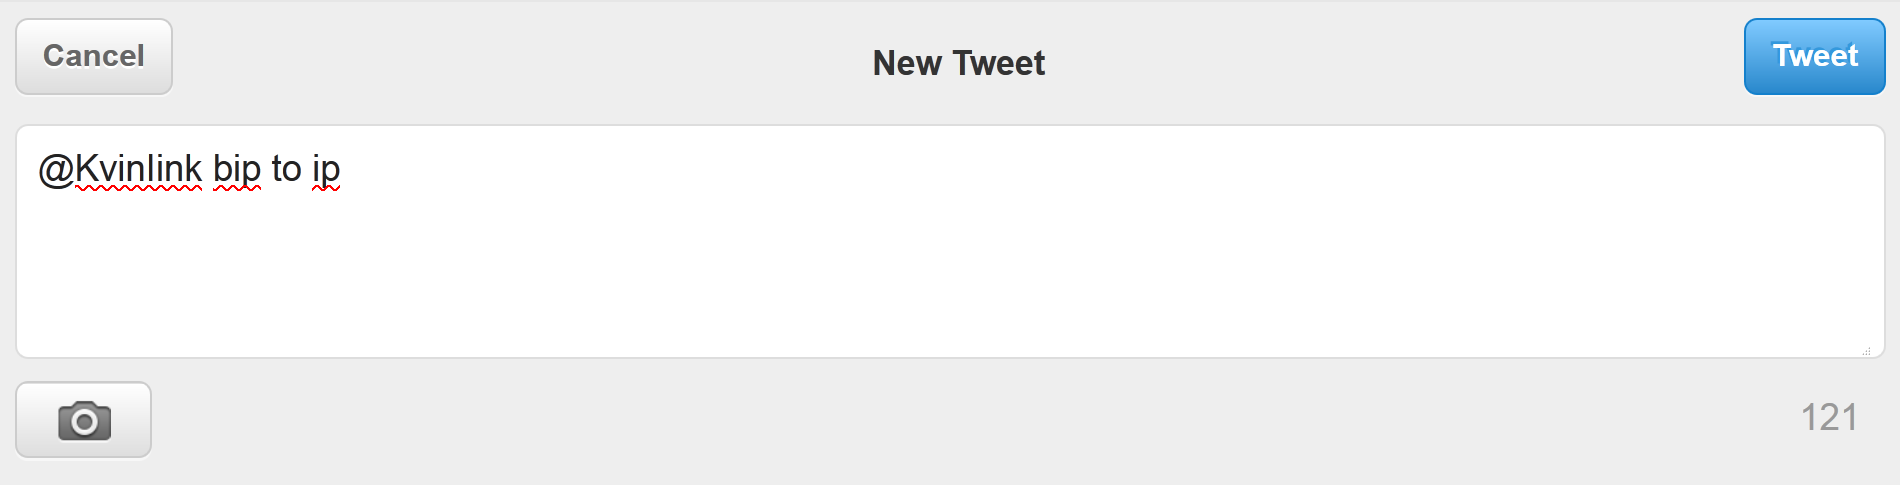
\includegraphics[width=0.75\textwidth]{C:/Skripsi/doc/DokumenSkripsi/Gambar/Tweet1.PNG}
		\caption{Tweet dari BIP menuju IP}
		\label{fig:Tweet1}
	\end{figure}
	
	Setelah proses \textit{tweet} dilakukan, \textit{Twitter bot} akan menangkap \textit{tweet} tersebut dan memprosesnya. Setelah proses pencarian selesai dilakukan, akun \textit{Twitter bot} @kviniink melakukan \textit{reply} kepada akun @kviniinktest123 yang dapat dilihat pada Gambar~\ref{fig:HasilTweet1}. 
	
		
	\begin{figure}
		\centering
			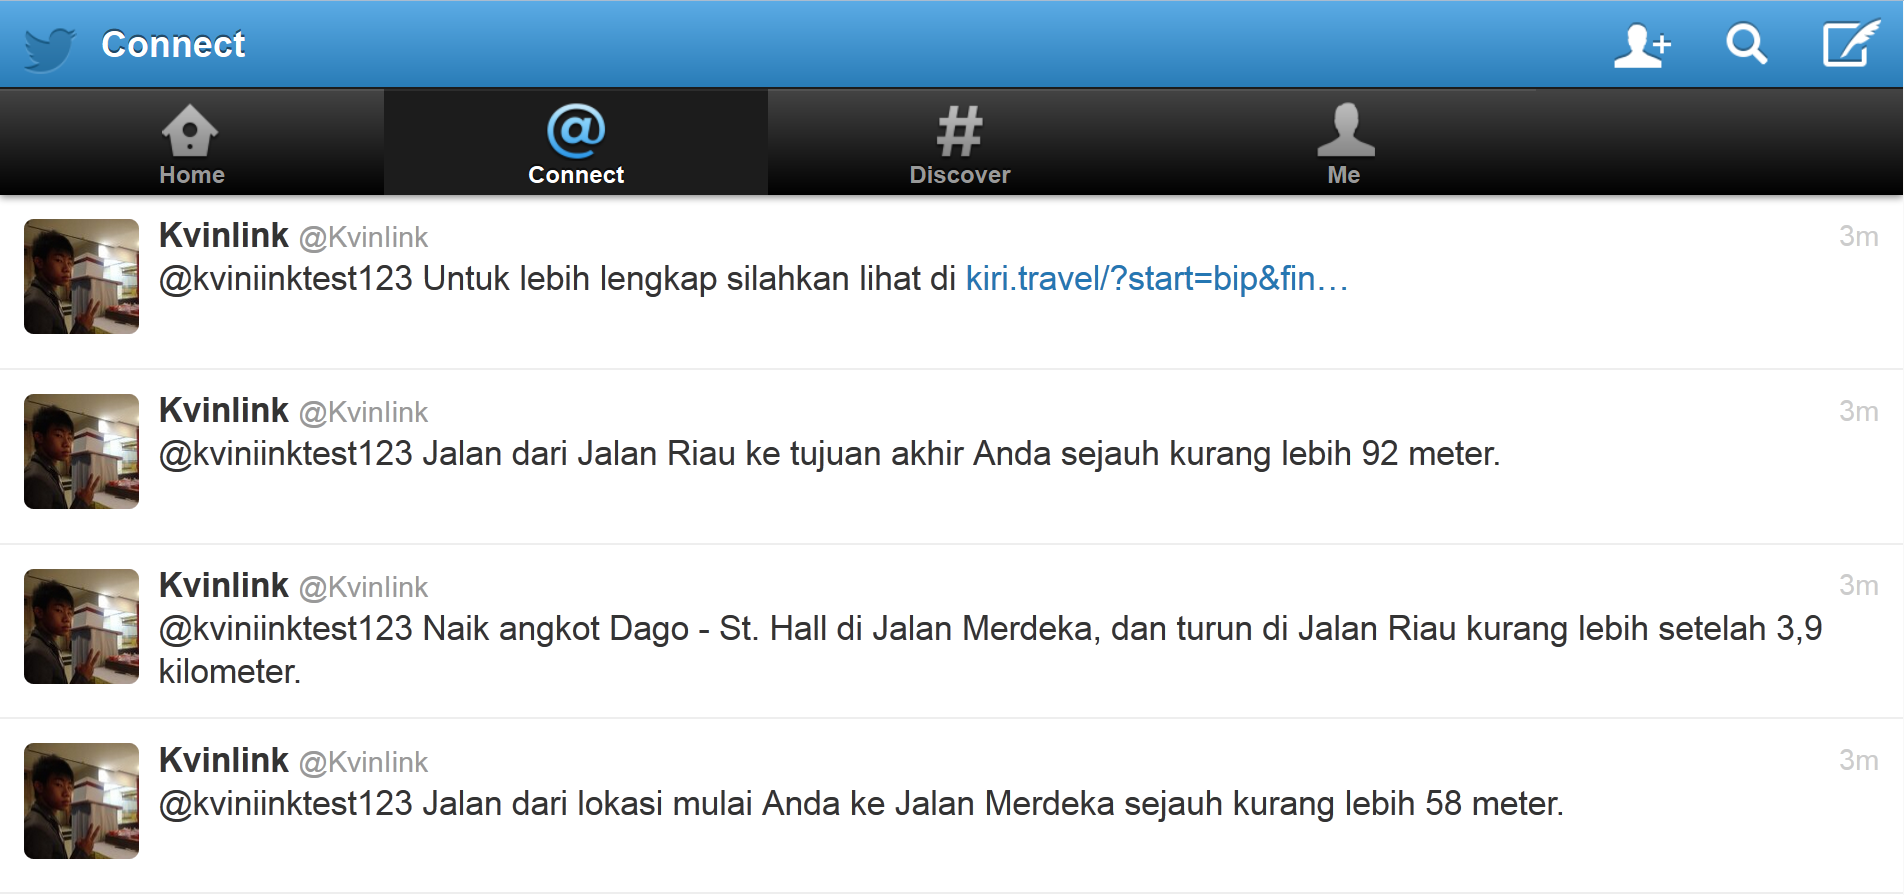
\includegraphics[width=0.75\textwidth]{C:/Skripsi/doc/DokumenSkripsi/Gambar/HasilTweet1.PNG}
		\caption{Hasil Pencarian Rute Transportasi Publik dari BIP menuju IP}
		\label{fig:HasilTweet1}
	\end{figure}
	
	Pencarian kedua dilakukan dengan lokasi awal yaitu BIP (Bandung Indah Plaza) dan lokasi tujuan yaitu PVJ (Paris van Java). Dapat dilihat pada Gambar~\ref{fig:Tweet2}, akun @kviniinktest123 melakukan \textit{tweet} pencarian jalur transportasi publik yang di-\textit{mention} kepada akun \textit{Twitter bot} @kviniink dengan lokasi awal yaitu BIP dan lokasi tujuan yaitu PVJ.
	
	\begin{figure}
		\centering
			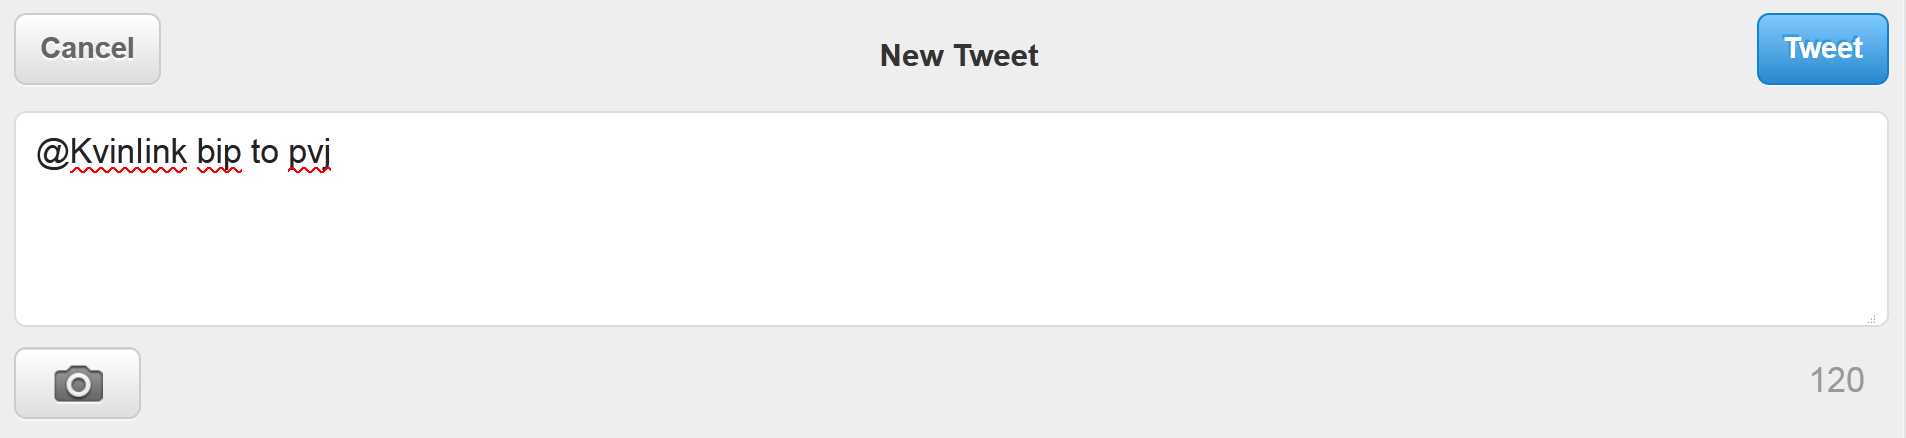
\includegraphics[width=0.75\textwidth]{C:/Skripsi/doc/DokumenSkripsi/Gambar/Tweet2.PNG}
		\caption{\textit{Tweet} dari BIP menuju PVJ}
		\label{fig:Tweet2}
	\end{figure}
	
	Setelah itu \textit{tweet} tersebut diproses oleh aplikasi untuk dicari jalur transportasi publiknya, lalu akun \textit{Twitter bot} @kviniink melakukan \textit{reply} kepada akun @kviniinktest123. \textit{Reply tweet} tersebut merupakan jalur transportasi publik yang harus ditempuh, \textit{reply tweet} tersebut dapat dilihat pada Gambar~\ref{fig:HasilTweet2}.
	
	
	\begin{figure}
		\centering
			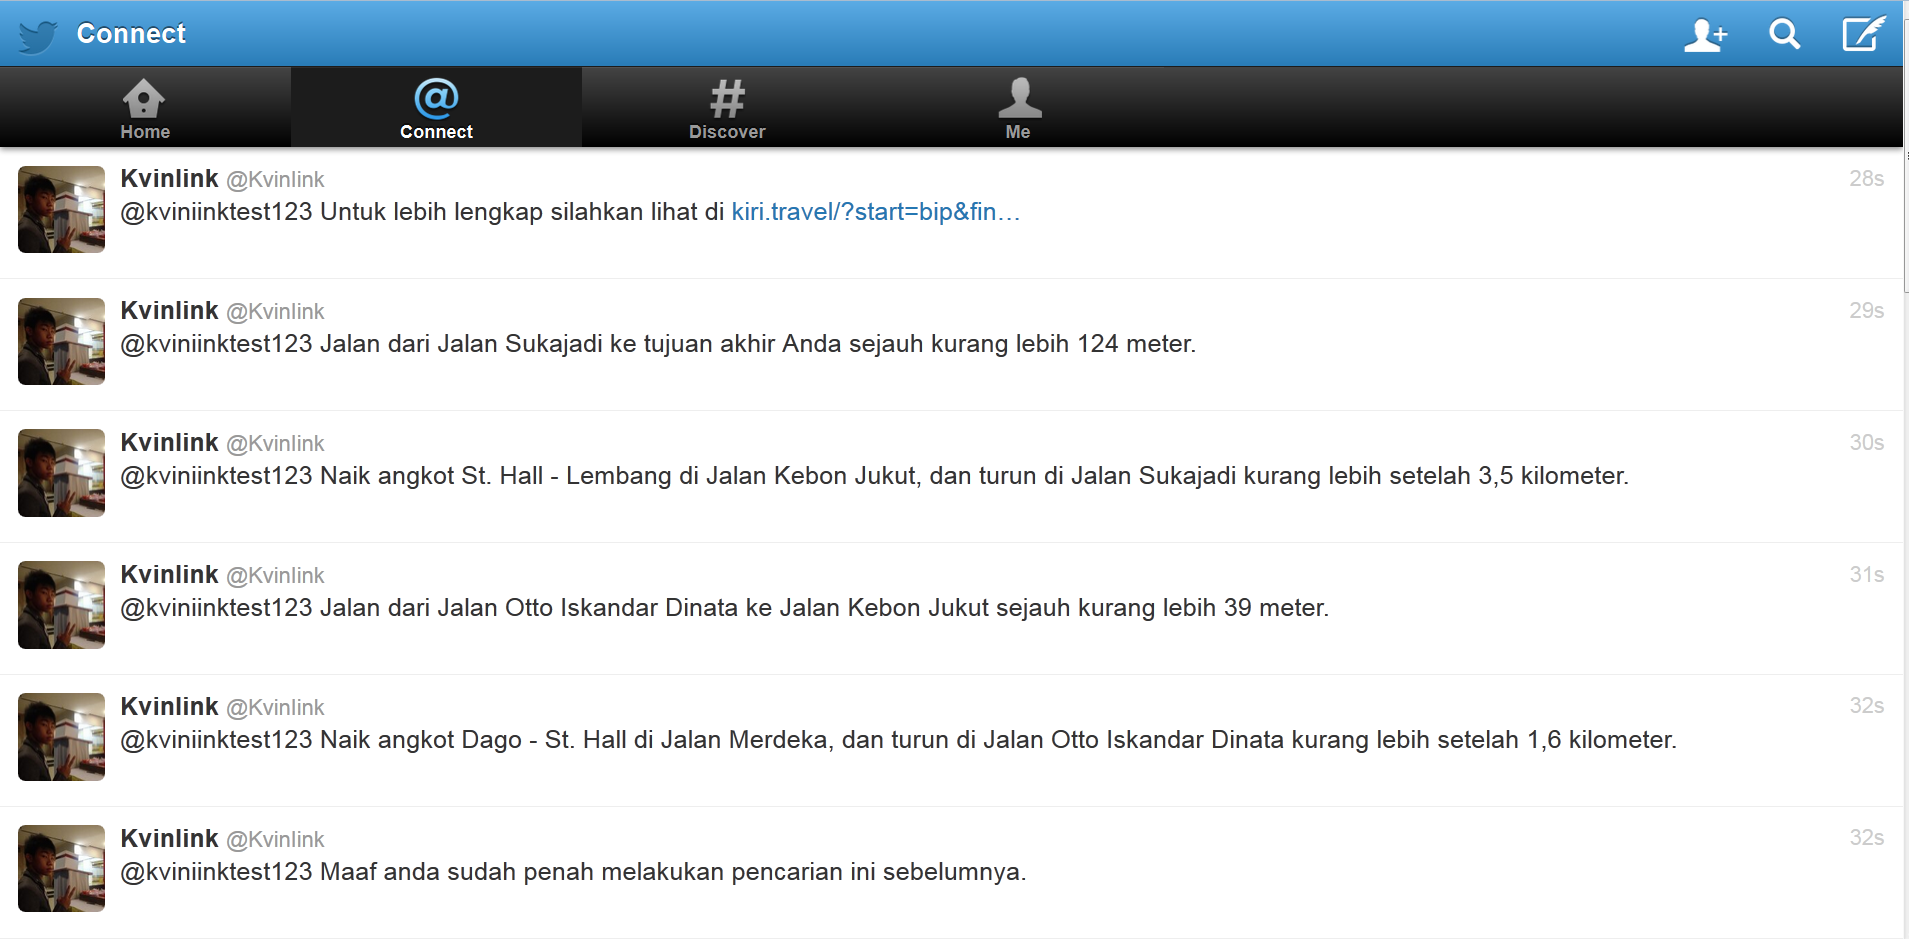
\includegraphics[width=0.75\textwidth]{C:/Skripsi/doc/DokumenSkripsi/Gambar/HasilTweet2.PNG}
		\caption{Hasil Pencarian Rute Transportasi Publik dari BIP menuju PVJ}
		\label{fig:HasilTweet2}
	\end{figure}
	
	Pada pencarian kedua dapat dilihat pada \textit{tweet} pertama terjadi ketidak sesuaian hasil dari KIRI API dengan hasil \textit{tweet}.
	Peneliti lalu melakukan pencarian melalui \textit{website} KIRI yaitu \url{http://kiri.travel}. Pencarian pertama pada \textit{website} KIRI dilakukan dengan lokasi awal yaitu BIP dan lokasi tujuan yaitu IP. Hasil pencarian pada \textit{website} KIRI dapat dilihat pada Gambar~\ref{fig:HasilKiri1}.
	
	
	\begin{figure}
		\centering
			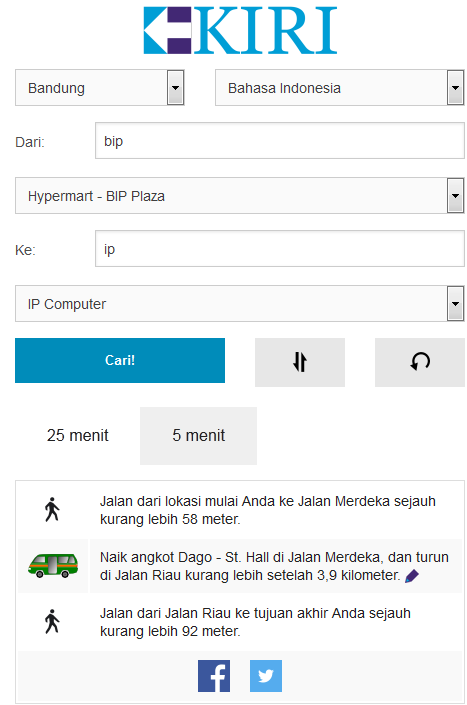
\includegraphics[width=0.5\textwidth]{C:/Skripsi/doc/DokumenSkripsi/Gambar/HasilKiri1.PNG}
		\caption{Hasil Pencarian Jalur Transportasi Publik dari BIP menuju IP Melalui Website KIRI}
		\label{fig:HasilKiri1}
	\end{figure}
	
	Lalu pencarian kedua pada \textit{website} KIRI dilakukan dengan lokasi awal yaitu BIP dan lokasi tujuan yaitu PVJ. Hasil pencarian KIRI dari BIP menuju PVJ dapat dilihat pada Gambar~\ref{fig:HasilKiri2}. Setelah dilihat dari hasil keduanya, \textit{Twitter bot} melakukan \textit{duplicate tweet} pada \textit{tweet} pertama dalam pencarian ke dua yang dilakukan oleh akun @kviniink123. \textit{Duplicate tweet} adalah \textit{tweet} yang dinyatakan dinyatakan identik oleh Twitter dalam jangka waktu tertentu. \textit{Duplicate tweet} tidak diperbolehkan oleh Twitter. Oleh karena itu, untuk menghindari adanya \textit{duplicate tweet}, penulis menambahkan waktu untuk jam, menit, dan detik di setiap \textit{tweet} yang dilakukan oleh \textit{Twitter bot} agar membuat setiap \textit{tweet} tersebut bersifat unik.
	
	\begin{figure}
		\centering
			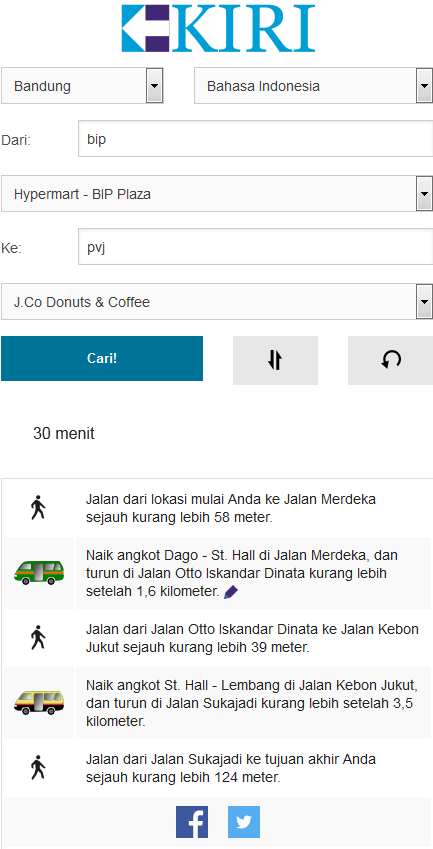
\includegraphics[width=0.5\textwidth]{C:/Skripsi/doc/DokumenSkripsi/Gambar/HasilKiri2.PNG}
		\caption{Hasil Pencarian Jalur Transportasi Publik dari BIP menuju PVJ Melalui Website KIRI}
		\label{fig:HasilKiri2}
	\end{figure}
	\clearpage
	
	\item Pengujian 1.1
	
	Pada pengujian satu, peneliti mencoba untuk mencari jalur transportasi publik untuk lokasi yang umum dikunjungi yaitu \textit{mall}. Pencarian dilakukan dengan lokasi awal yaitu PVJ (Paris Van Java) menuju lokasi tujuan yaitu BIP (Bandung Indah Plaza). Akun penguji @kviniinktest123 melakukan \textit{mention} kepada akun \textit{Twitter bot} @kviniink123 yang dapat dilihat pada Gambar~\ref{fig:Tweet1_1}.
	
	\begin{figure}
		\centering
			
\includegraphics[width=0.75\textwidth]{C:/Skripsi/doc/DokumenSkripsi/Gambar/Tweet1_1.PNG}
		\caption{Tweet dari PVJ menuju BIP}
		\label{fig:Tweet1_1}
	\end{figure}
	
	Setelah proses \textit{tweet} dilakukan, \textit{Twitter bot} akan menangkap \textit{tweet} tersebut dan memprosesnya. Setelah proses pencarian selesai dilakukan, akun \textit{Twitter bot} @kviniink melakukan \textit{reply} kepada akun @kviniinktest123 yang dapat dilihat pada Gambar~\ref{fig:HasilTweet1_1}. 
	
		
	\begin{figure}
		\centering
			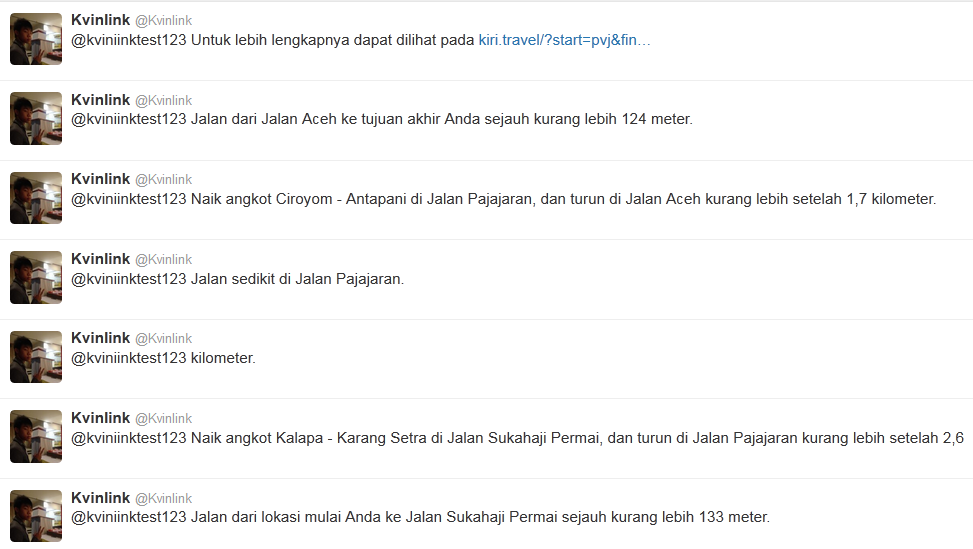
\includegraphics[width=0.75\textwidth]{C:/Skripsi/doc/DokumenSkripsi/Gambar/HasilTweet1_1.PNG}
		\caption{Hasil Pencarian Rute Transportasi Publik dari BIP menuju IP}
		\label{fig:HasilTweet1_1}
	\end{figure}
	
	Pencarian kedua dilakukan dengan lokasi awal yaitu PVJ(Paris Van Java) dan lokasi tujuan yaitu Museum KAA(Konferensi Asia Afrika). Dapat dilihat pada Gambar~\ref{fig:Tweet2_2}, akun @kviniinktest123 melakukan \textit{tweet} pencarian jalur transportasi publik yang di-\textit{mention} kepada akun \textit{Twitter bot} @kviniink dengan lokasi awal yaitu PVJ dan lokasi tujuan yaitu Museum KAA.
	
	\begin{figure}
		\centering
			
\includegraphics[width=0.75\textwidth]{C:/Skripsi/doc/DokumenSkripsi/Gambar/Tweet2_2.PNG}
		\caption{\textit{Tweet} dari PVJ menuju Museum KAA}
		\label{fig:Tweet2_2}
	\end{figure}
	
	Setelah itu \textit{tweet} tersebut diproses oleh aplikasi untuk dicari jalur transportasi publiknya, lalu akun \textit{Twitter bot} @kviniink melakukan \textit{reply} kepada akun @kviniinktest123. \textit{Reply tweet} tersebut merupakan jalur transportasi publik yang harus ditempuh, \textit{reply tweet} tersebut dapat dilihat pada Gambar~\ref{fig:HasilTweet2_2}.
	
	
	\begin{figure}
		\centering
			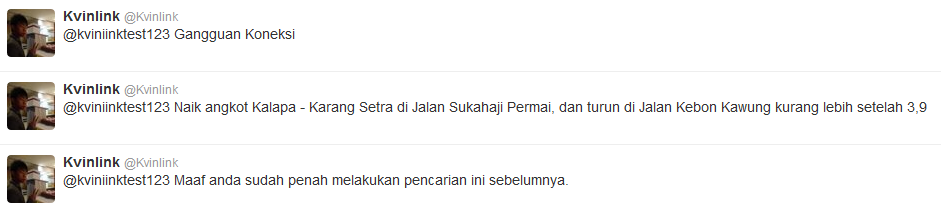
\includegraphics[width=0.75\textwidth]{C:/Skripsi/doc/DokumenSkripsi/Gambar/HasilTweet2_2.PNG}
		\caption{Hasil Pencarian Rute Transportasi Publik dari PVJ menuju Museum KAA}
		\label{fig:HasilTweet2_2}
	\end{figure}
	
	Pada pencarian kedua dapat dilihat pada \textit{tweet} pertama terjadi ketidak sesuaian hasil dari KIRI API dengan hasil \textit{tweet}.
	Peneliti lalu melakukan pencarian melalui \textit{website} KIRI yaitu \url{http://kiri.travel}. Pencarian pertama pada \textit{website} KIRI dilakukan dengan lokasi awal yaitu PVJ dan lokasi tujuan yaitu BIP. Hasil pencarian pada \textit{website} KIRI dapat dilihat pada Gambar~\ref{fig:HasilKiri1}.
	
	
	\begin{figure}
		\centering
			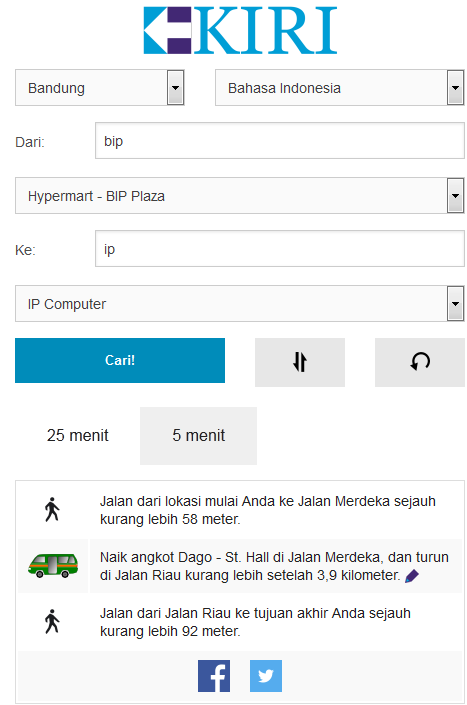
\includegraphics[width=0.5\textwidth]{C:/Skripsi/doc/DokumenSkripsi/Gambar/HasilKiri1.PNG}
		\caption{Hasil Pencarian Jalur Transportasi Publik dari BIP menuju IP Melalui Website KIRI}
		\label{fig:HasilKiri1}
	\end{figure}
	
	Lalu pencarian kedua pada \textit{website} KIRI dilakukan dengan lokasi awal yaitu PVJ dan lokasi tujuan yaitu Museum KAA. Hasil pencarian KIRI dari PVJ menuju Museum KAA dapat dilihat pada Gambar~\ref{fig:HasilKiri2}. Setelah dilihat dari hasil keduanya, \textit{Twitter bot} melakukan \textit{duplicate tweet} pada \textit{tweet} pertama dalam pencarian ke dua yang dilakukan oleh akun @kviniink123. \textit{Duplicate tweet} adalah \textit{tweet} yang dinyatakan dinyatakan identik oleh Twitter dalam jangka waktu tertentu. \textit{Duplicate tweet} tidak diperbolehkan oleh Twitter. Oleh karena itu, untuk menghindari adanya \textit{duplicate tweet}, penulis menambahkan waktu untuk jam, menit, dan detik di setiap \textit{tweet} yang dilakukan oleh \textit{Twitter bot} agar membuat setiap \textit{tweet} tersebut bersifat unik.
	
	\begin{figure}
		\centering
			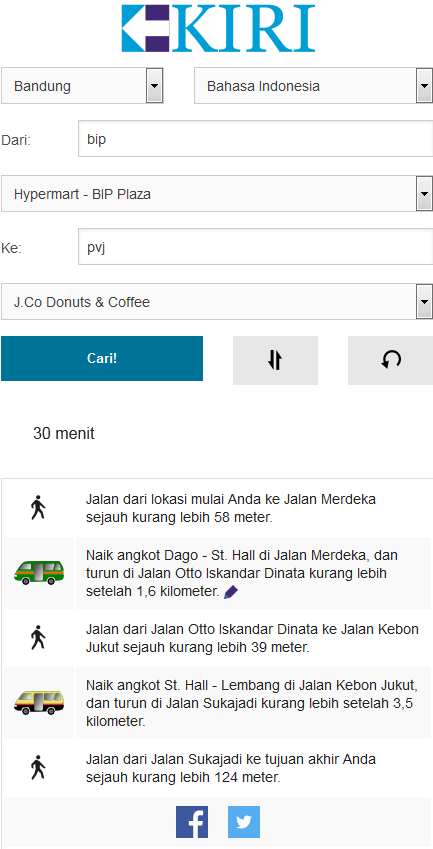
\includegraphics[width=0.5\textwidth]{C:/Skripsi/doc/DokumenSkripsi/Gambar/HasilKiri2.PNG}
		\caption{Hasil Pencarian Jalur Transportasi Publik dari BIP menuju PVJ Melalui Website KIRI}
		\label{fig:HasilKiri2}
	\end{figure}
	\clearpage
	
	\item Pengujian 2
	
	Pada pengujian dua, penulis melakukan pengujian dengan cara menjalankan aplikasi selama 24 jam. Selain itu penulis juga melakukan pengujian dengan cara meminta bantuan kepada beberapa responden untuk melakukan \textit{tweet} pencarian jalur transportasi publik. Pengujian ini dilakukan untung mengetahui apakah aplikasi \textit{Twitter bot} berjalan dengan baik atau tidak. Dari hasil yang didapatkan \textit{Twitter bot} dapat memberi pesan bahwa suatu lokasi pencarian tidak ditemukan. Pesan pemberitahuan yang dapat dilihat pada Gambar~\ref{fig:HasilFinal1}. Selain itu juga \textit{Twitter bot} dapat memberi pesan juga lokasi awal dan lokasi tujuan merupakan lokasi yang sama. Pesan pemberitahuan dapat dilihat pada Gambar~\ref{fig:HasilTweetSama}.
	Pada Gambar~\ref{fig:HasilFinal1} dapat dilihat bahwa akun @cla\_amour mencari lokasi tki dan kopo tetapi lokasi pencarian tidak ditemukan. Akun @cla\_amour juga mencari jalur transportasi publik yang lokasinya ditemukan tetapi tidak ada rute transportasi publiknya. Hasil \textit{reply Twitter bot} yang dilakukan oleh akun @cla\_amour dapat dilihat pada salah satu \textit{reply} yang terdapat pada Gambar~\ref{fig:HasilFinal1}.
	
	Selain itu \textit{Twitter bot} tidak akan mendapatkan \textit{error} ketika akun \textit{Twitter Bot} @kviniink mendapat banyak \textit{mention} dalam satu \textit{tweet} seperti pada Gambar~\ref{fig:testTweet}, jika format penulisan benar maka \textit{Twitter bot} akan tetap mencari jalur transportasi publiknya yang dapat dilihat pada Gambar~\ref{fig:hasilTestTweet}. 
	Gambar~\ref{fig:HasilFinal1}, Gambar~\ref{fig:HasilFinal2}, dan Gambar~\ref{fig:HasilFinal3} merupakan beberapa hasil \textit{reply} dari \textit{Twitter bot}.
	
	\newpage
	\begin{figure}
		\centering
			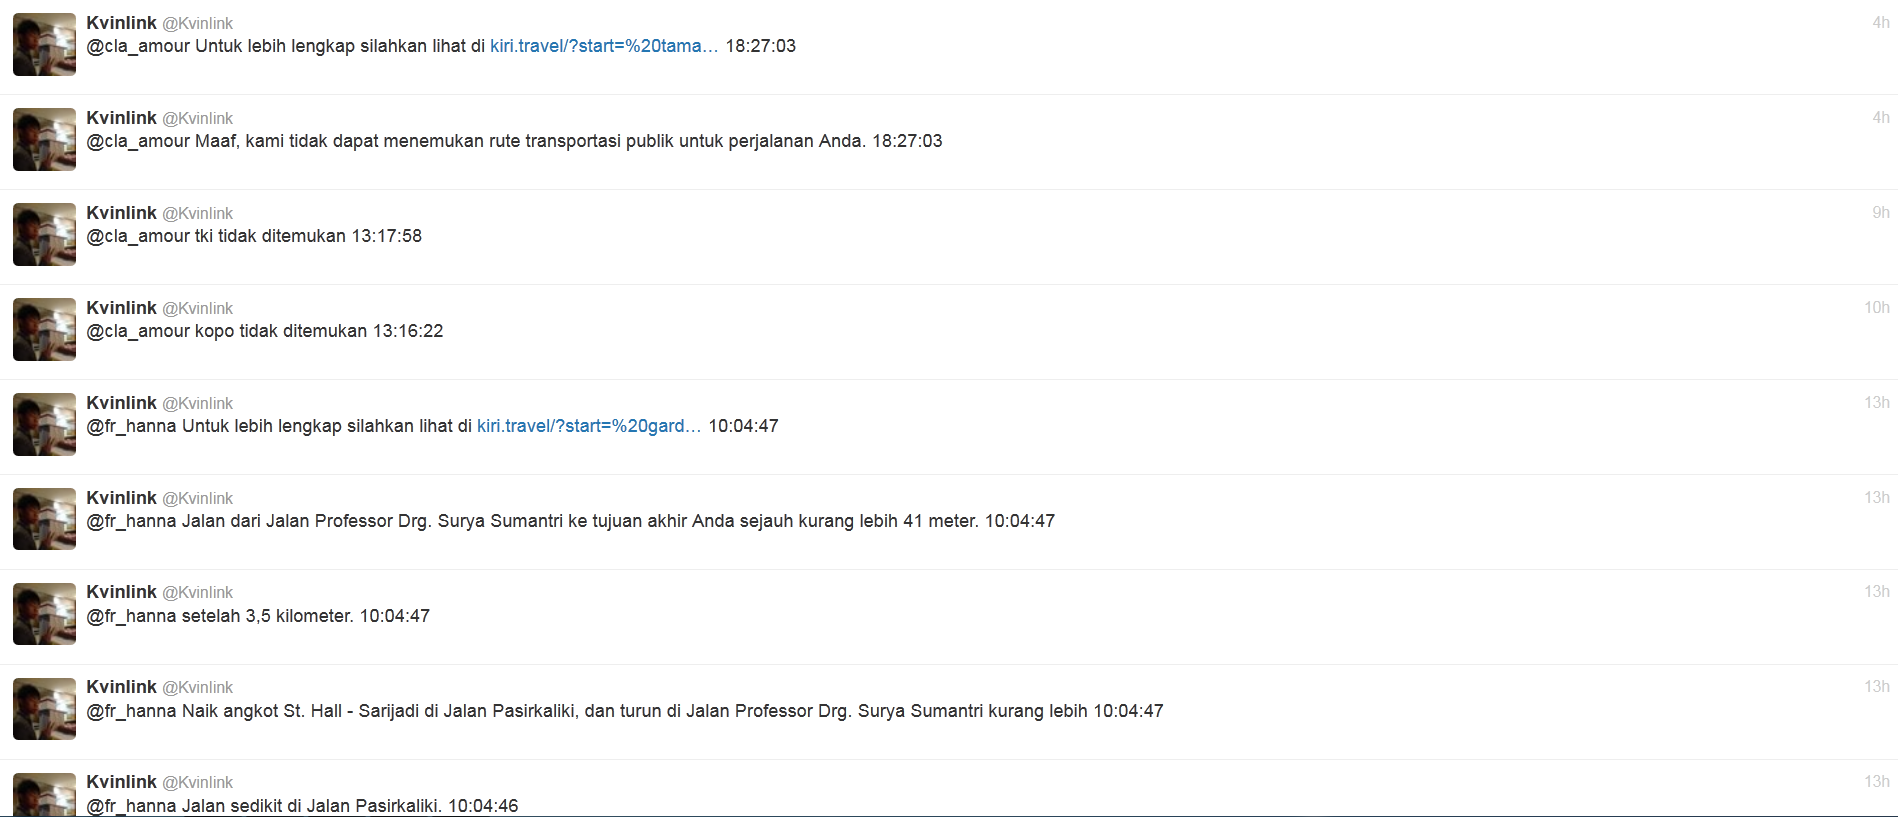
\includegraphics[width=0.9\textwidth]{C:/Skripsi/doc/DokumenSkripsi/Gambar/HasilFinal1.PNG}
		\caption{Hasil Reply Twitter Bot}
		\label{fig:HasilFinal1}
	\end{figure}
	
	\begin{figure}
		\centering
			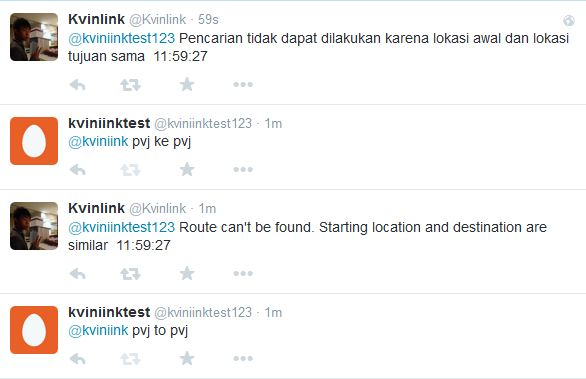
\includegraphics[width=0.9\textwidth]{C:/Skripsi/doc/DokumenSkripsi/Gambar/HasilTweetSama.JPG}
		\caption{Hasil \textit{Tweet} Jika Lokasi Awal dan Lokasi Tujuan Sama}
		\label{fig:HasilTweetSama}
	\end{figure}
	
	\begin{figure}
		\centering
			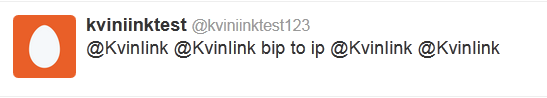
\includegraphics[width=0.9\textwidth]{C:/Skripsi/doc/DokumenSkripsi/Gambar/testTweet.PNG}
		\caption{Akun \textit{Twitter Bot} Mendapat Banyak Mention Dalam Satu \textit{Tweet}}
		\label{fig:testTweet}
	\end{figure}
	
	\begin{figure}
		\centering
			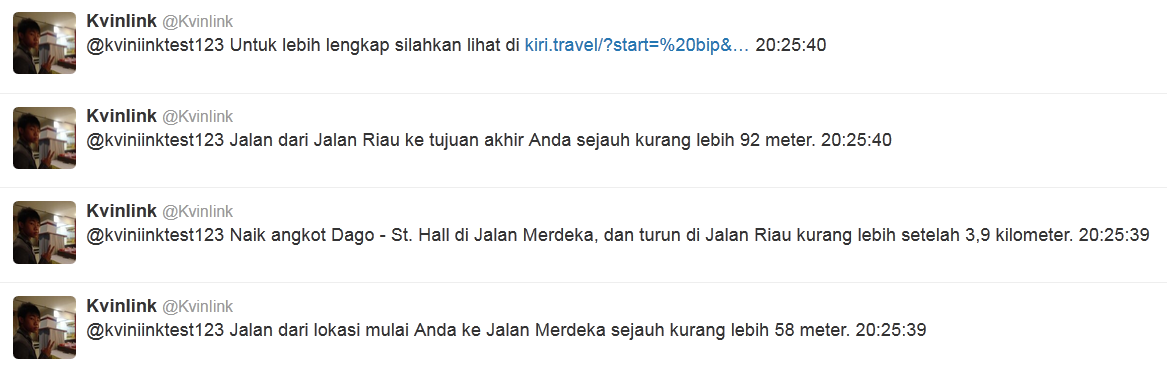
\includegraphics[width=0.9\textwidth]{C:/Skripsi/doc/DokumenSkripsi/Gambar/hasilTestTweet.PNG}
		\caption{Hasil Reply \textit{Twitter Bot}}
		\label{fig:hasilTestTweet}
	\end{figure}
	
	\begin{figure}
		\centering
			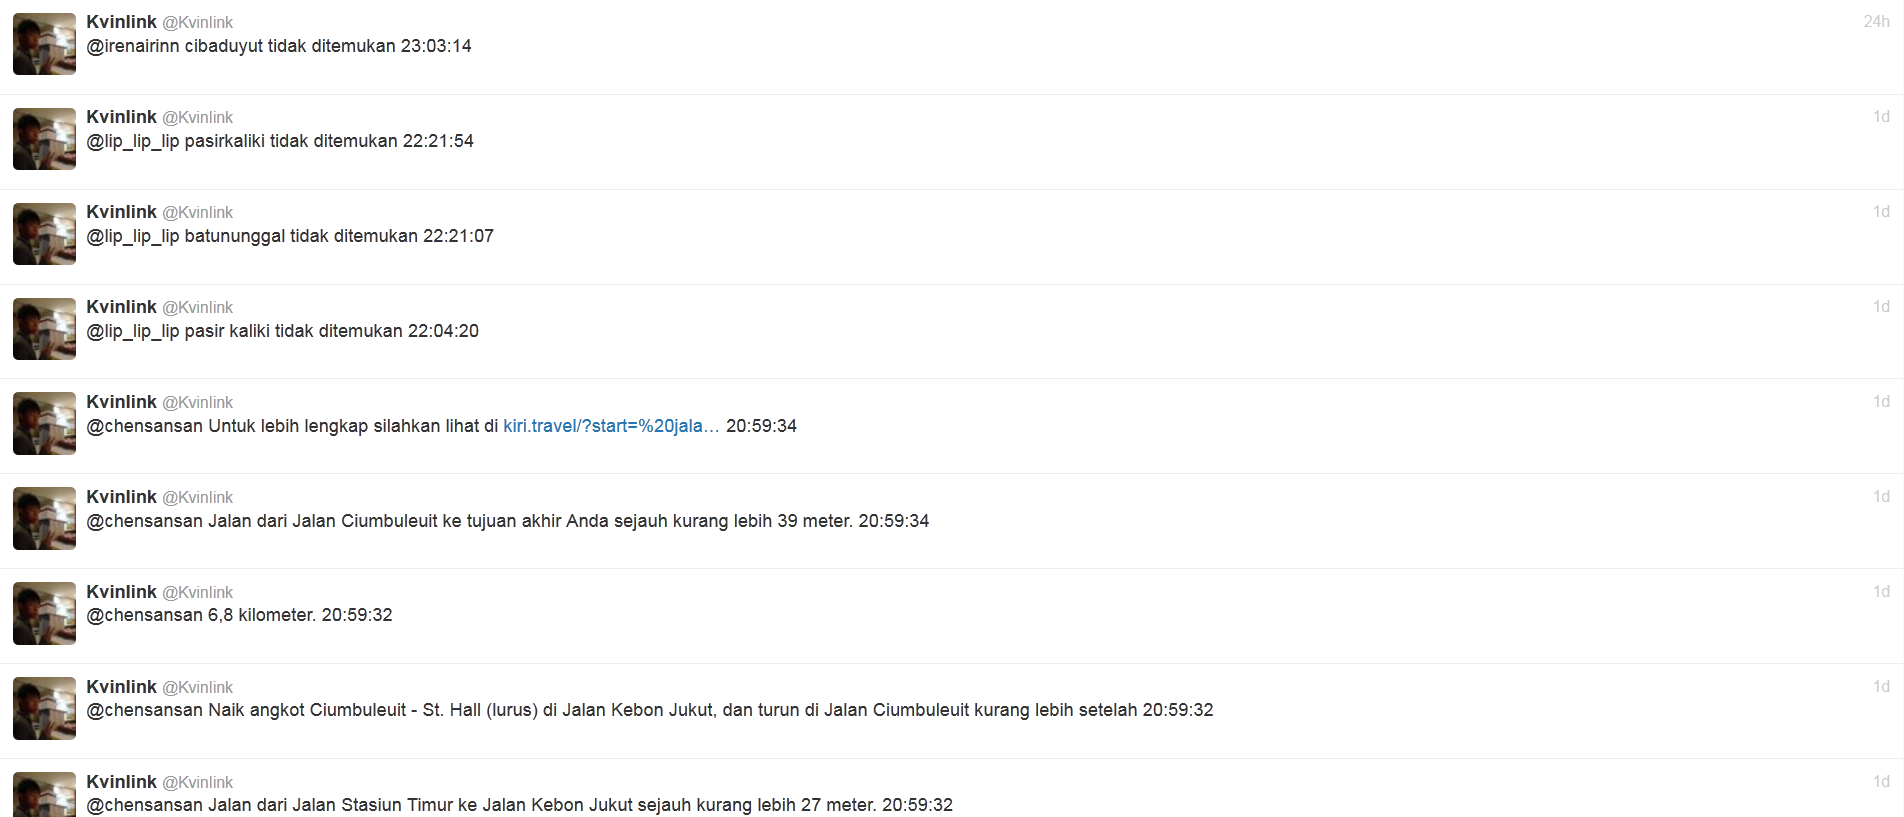
\includegraphics[width=0.9\textwidth]{C:/Skripsi/doc/DokumenSkripsi/Gambar/HasilFinal2.PNG}
			\caption{Hasil Reply \textit{Twitter Bot}}
		\label{fig:HasilFinal2}
	\end{figure}
	
	\begin{figure}
		\centering
			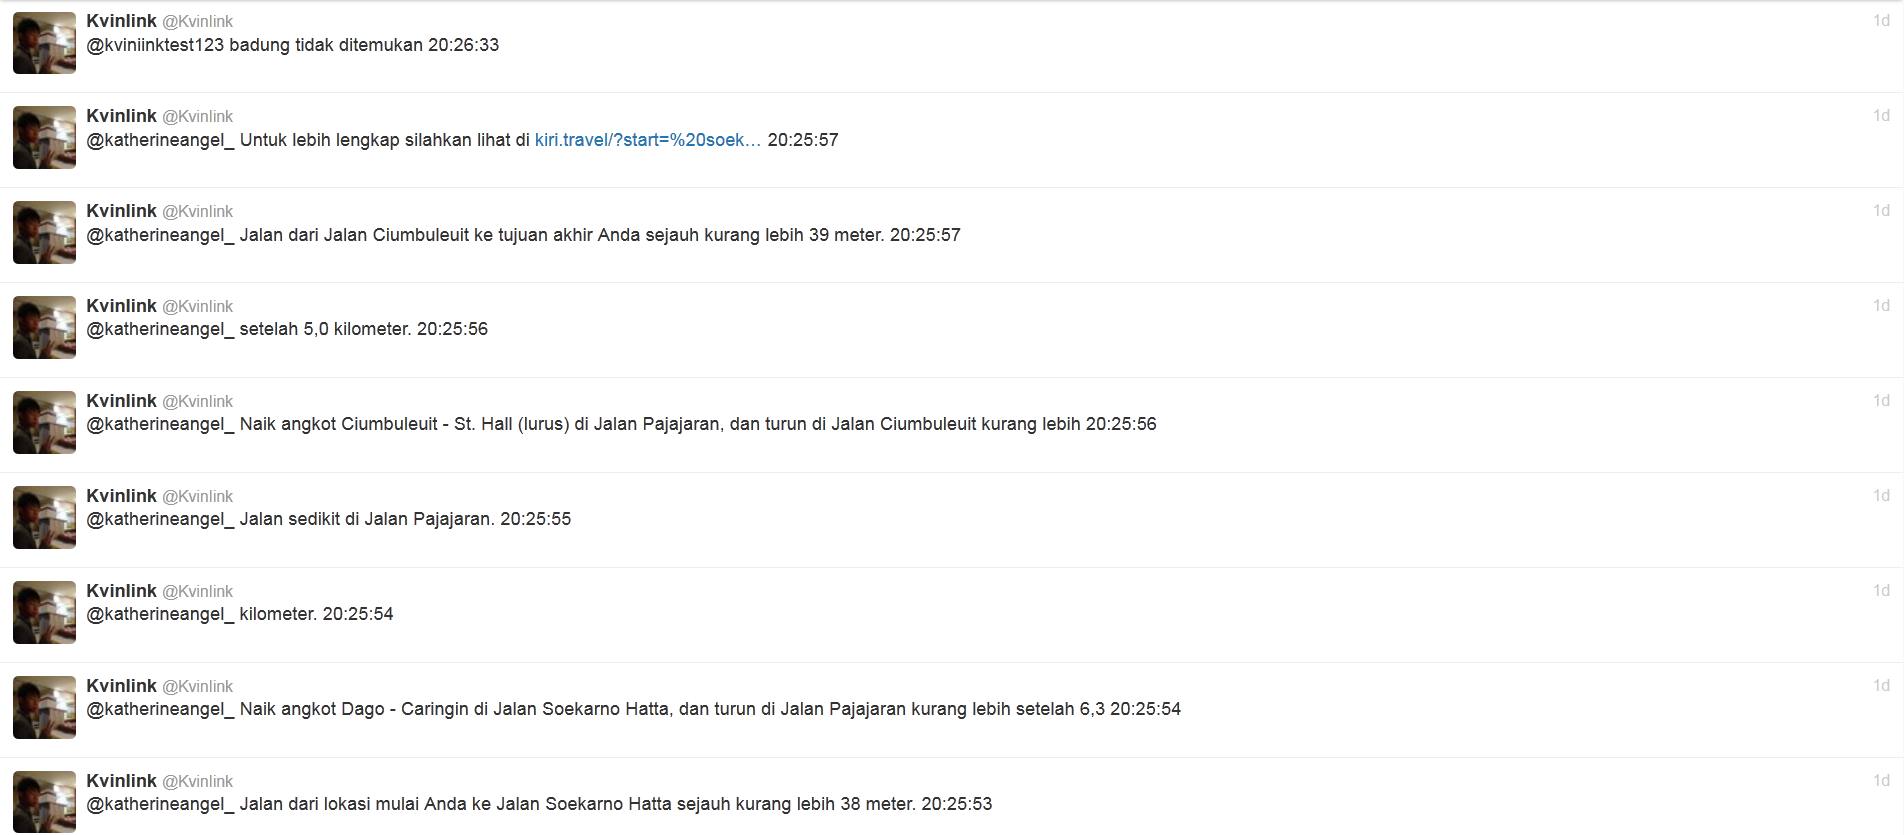
\includegraphics[width=0.9\textwidth]{C:/Skripsi/doc/DokumenSkripsi/Gambar/HasilFinal3.PNG}
			\caption{Hasil Reply \textit{Twitter Bot}}
		\label{fig:HasilFinal3}
	\end{figure}
	
	\clearpage
	\item Pengujian 3
	
	Pada pengujian tiga dilakukan pengujian untuk mengetahui apakah hasil \textit{tweet} yang diberikan \textit{Twitter bot} terdapat kesalahan atau tidak jika \textit{Twitter bot} mendapatkan dua \textit{tweet} atau lebih pada waktu yang bersamaan. Pengujian dilakukan dengan cara melakukan dua \textit{tweet} pencarian secara bersamaan. Penulis meminta bantuan kepada beberapa responden untuk melakukan \textit{tweet} pencarian secara bersamaan. Hasil pengujian untuk \textit{tweet} pencarian yang dilakukan secara bersamaan dapat dilihat pada tabel~\ref{tab:tabelHasilPengujianTweetYangDilakukanSecaraBersamaan}.
	
	\begin{table}[h]
	\caption{Tabel 1 hasil pengujian \textit{tweet} yang dilakukan secara bersamaan}
	\label{tab:tabelHasilPengujianTweetYangDilakukanSecaraBersamaan}
		\begin{tabular}{|p{0.5cm}|p{2.5cm}|p{1.5cm}|p{4cm}|p{6cm}|}
			\hline
				No & Akun penguji & Waktu \textit{tweet} & \textit{Tweet} yang dikirimkan pengguna & \textit{Tweet} yang diterima pengguna \\ \hline
				1 & @ClaraKwaria & 10:49 &  @KvinIink UNPAR to PVJ & 
				\begin{itemize}
					\item @ClaraKwaria Walk about 44 meter from your starting point to Jalan Ciumbuleuit. 22:49:19
					\item @ClaraKwaria Take angkot Ciumbuleuit - St. Hall (belok) at Jalan Ciumbuleuit, and alight at Jalan Sederhana about 2.4 kilometer 22:49:20
					\item @ClaraKwaria later. 22:49:20
					\item @ClaraKwaria Walk about 460 meter from Jalan Sederhana to your destination. 22:49:20
					\item @ClaraKwaria For futher information you can visit http:\/\/kiri.travel?start=unpar \&finish=pvj\&region=bdo 22:49:20
				\end{itemize} \\ \hline
				2 & @clara00010111 & 10:49 &  @KvinIink UNPAR to PVJ &
				\begin{itemize}
					\item @clara00010111 Walk about 44 meter from your starting point to Jalan Ciumbuleuit. 22:49:23 
					\item @clara00010111 Take angkot Ciumbuleuit - St. Hall (belok) at Jalan Ciumbuleuit, and alight at Jalan Sederhana about 2.4 kilometer 22:49:23
					\item @clara00010111 later. 22:49:23
					\item @clara00010111 Walk about 460 meter from Jalan Sederhana to your destination. 22:49:24
					\item @clara00010111 For futher information you can visit http:\/\/kiri.travel?start=unpar \&finish=pvj\&region=bdo 22:49:24
				\end{itemize} \\ \hline
		\end{tabular}
\end{table}

\begin{table}[h]
	\caption{Tabel 2 hasil pengujian \textit{tweet} yang dilakukan secara bersamaan}
	\label{tab:tabelHasilPengujianTweetYangDilakukanSecaraBersamaan}
		\begin{tabular}{|p{0.5cm}|p{2.5cm}|p{1.5cm}|p{4cm}|p{6cm}|}
			\hline
				No & Akun penguji & Waktu \textit{tweet} & \textit{Tweet} yang dikirimkan pengguna & \textit{Tweet} yang diterima pengguna \\ \hline
				3 & @ClaraKwaria & 10:52 &  @KvinIink UNPAR ke PVJ &
				\begin{itemize}
					\item @clara00010111 Jalan dari lokasi mulai Anda ke Jalan Ciumbuleuit sejauh kurang lebih 44 meter. 22:52:37
					\item @clara00010111 Naik angkot Ciumbuleuit - St. Hall (belok) di Jalan Ciumbuleuit, dan turun di Jalan Sederhana kurang lebih setelah 22:52:38
					\item @clara00010111 2,4 kilometer. 22:52:38
					\item @clara00010111 Jalan dari Jalan Sederhana ke tujuan akhir Anda sejauh kurang lebih 460 meter. 22:52:39
					\item @clara00010111 Untuk lebih lengkapnya dapat dilihat pada http:\/\/kiri.travel?start=unpar \&finish=pvj\&region=bdo 22:52:39 
				\end{itemize} \\ \hline
				4 & @clara00010111 & 10:52 &  @KvinIink UNPAR ke PVJ &
				\begin{itemize}
					\item @clara00010111 Jalan dari lokasi mulai Anda ke Jalan Ciumbuleuit sejauh kurang lebih 44 meter. 22:52:34
					\item @clara00010111 Naik angkot Ciumbuleuit - St. Hall (belok) di Jalan Ciumbuleuit, dan turun di Jalan Sederhana kurang lebih setelah 22:52:34
					\item @clara00010111 2,4 kilometer. 22:52:34
					\item @clara00010111 Jalan dari Jalan Sederhana ke tujuan akhir Anda sejauh kurang lebih 460 meter. 22:52:35
					\item @clara00010111 Untuk lebih lengkapnya dapat dilihat pada http:\/\/kiri.travel?start=unpar \&finish=pvj\&region=bdo 22:52:35 
				\end{itemize} \\ \hline
		\end{tabular}
\end{table}

\begin{table}[h]
	\caption{Tabel 3 hasil pengujian \textit{tweet} yang dilakukan secara bersamaan}
	\label{tab:tabelHasilPengujianTweetYangDilakukanSecaraBersamaan}
		\begin{tabular}{|p{0.5cm}|p{2.5cm}|p{1.5cm}|p{4cm}|p{6cm}|}
			\hline
				No & Akun penguji & Waktu \textit{tweet} & \textit{Tweet} yang dikirimkan pengguna & \textit{Tweet} yang diterima pengguna \\ \hline
				5 & @ClaraKwaria & 10:59 &  @KvinIink UNPAR ke BIP &
				\begin{itemize}
					\item @ClaraKwaria Jalan dari lokasi mulai Anda ke Jalan Ciumbuleuit sejauh kurang lebih 44 meter. 23:00:04
					\item @ClaraKwaria Naik angkot Ciumbuleuit - St. Hall (lurus) di Jalan Ciumbuleuit, dan turun di Jalan Cihampelas kurang lebih setelah 23:00:04
					\item @ClaraKwaria 3,3 kilometer. 23:00:04
					\item @ClaraKwaria Jalan dari Jalan Cihampelas ke Jalan Wastukancana sejauh kurang lebih 17 meter. 23:00:05
					\item @ClaraKwaria Naik angkot Ciroyom - Antapani di Jalan Wastukancana, dan turun di Jalan Aceh kurang lebih setelah 1,4 kilometer. 23:00:06
					\item @ClaraKwaria Jalan dari Jalan Aceh ke tujuan akhir Anda sejauh kurang lebih 124 meter. 23:00:06
					\item @ClaraKwaria Untuk lebih lengkapnya dapat dilihat pada http:\/\/kiri.travel?start=unpar \&finish=bip\&region=bdo 23:00:02 23:00:06
				\end{itemize} \\ \hline
		\end{tabular}
\end{table}

\begin{table}[h]
	\caption{Tabel 4 hasil pengujian \textit{tweet} yang dilakukan secara bersamaan}
	\label{tab:tabelHasilPengujianTweetYangDilakukanSecaraBersamaan}
		\begin{tabular}{|p{0.5cm}|p{2.5cm}|p{1.5cm}|p{4cm}|p{6cm}|}
			\hline
				No & Akun penguji & Waktu \textit{tweet} & \textit{Tweet} yang dikirimkan pengguna & \textit{Tweet} yang diterima pengguna \\ \hline
				6 & @clara00010111 & 10:59 &  @KvinIink UNPAR to BIP &
				\begin{itemize}
					\item @clara00010111 Walk about 44 meter from your starting point to Jalan Ciumbuleuit. 22:59:59
					\item @clara00010111 Take angkot Ciumbuleuit - St. Hall (lurus) at Jalan Ciumbuleuit, and alight at Jalan Cihampelas about 3.3 kilometer 23:00:00
					\item @clara00010111 later. 23:00:00
					\item @clara00010111 Walk about 17 meter from Jalan Cihampelas to Jalan Wastukancana. 23:00:01
					\item @clara00010111 Take angkot Ciroyom - Antapani at Jalan Wastukancana, and alight at Jalan Aceh about 1.4 kilometer later. 23:00:01
					\item @clara00010111 Walk about 124 meter from Jalan Aceh to your destination. 23:00:02
					\item @clara00010111 For futher information you can visit http:\/\/kiri.travel?start=unpar \&finish=bip\&region=bdo 23:00:02
				\end{itemize} \\ \hline
				7 & @ClaraKwaria & 10:02 &  @KvinIink bantuan &
				\begin{itemize}
					\item @ClaraKwaria Format penggunaan \textit{Twitter bot} untuk mencari jalur transportasi publik adalah... 23:00:06
					\item @ClaraKwaria 'Lokasi awal' ke 'lokasi tujuan', contoh : BIP ke PVJ. 23:00:06
				\end{itemize} \\ \hline
				8 & @clara00010111 & 10:02 &  @KvinIink help &
				\begin{itemize}
					\item @clara00010111 For using this \textit{Twitter bot} for searching public transport route, you can mention... 23:00:06
					\item @clara00010111 'First location' to 'second location', example : BIP to PVJ 23:00:06
				\end{itemize} \\ \hline
		\end{tabular}
\end{table}

\end{enumerate}